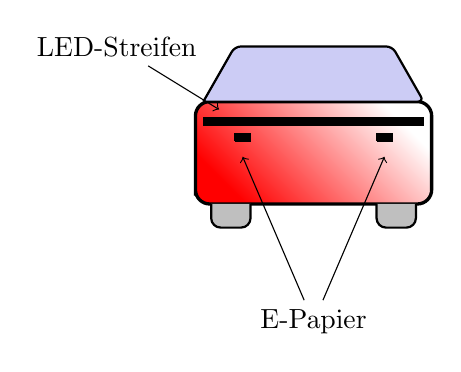
\begin{tikzpicture}
	\shade[top color=red, bottom color=white, shading angle={135}]
	[draw=black,fill=red!20,rounded corners=1.2ex,very thick] (1.5,0.5) -- ++(0,1.3) -- ++(3,0) -- ++(0,-1.3) -- (1.5,0.5) -- cycle;
	\draw[very thick, rounded corners=0.5ex,fill=black!20!blue!20!white,thick]  (1.6,1.8) -- ++(0.4,0.7) -- ++(2,0) -- ++(0.4,-0.7) -- (1.6,1.8);
	\node[] (S1) at (0.5, 2.5){LED-Streifen};
	\node[] (S2) at (3, -1){E-Papier};
	\draw[fill=black] (1.6,1.5) -- ++(2.8, 0) -- ++(0, 0.1) -- ++ (-2.8, 0) -- ++(0, -0.1);
	\draw[fill=black] (2,1.3) -- ++(0.2, 0) -- ++(0, 0.1) -- ++ (-0.2, 0) -- ++(0, -0.1);
	\draw[fill=black] (3.8,1.3) -- ++(0.2, 0) -- ++(0, 0.1) -- ++ (-0.2, 0) -- ++(0, -0.1);
	\draw[->] (S1) -- (1.8,1.7);
	\draw[->] (S2) -- (2.1, 1.1);
	\draw[->] (S2) -- (3.9, 1.1);
	\draw[draw=black,fill=gray!50,thick, rounded corners=0.8ex] 
	(1.7,0.5) -- ++(0,-0.3) -- ++(0.5, 0) -- ++(0,0.3);
	\draw[draw=black,fill=gray!50,thick, rounded corners=0.8ex] 
	(3.8,0.5) -- ++(0,-0.3) -- ++(0.5, 0) -- ++(0,0.3);
\end{tikzpicture}